% Slides made from README.tex
% compile with  pdflatex MilneMCslides.tex   (twice)
\documentclass[aspectratio=169,10pt]{beamer}
\usetheme{Boadilla}
\usecolortheme{beaver}
\usefonttheme[onlymath]{serif}
\setbeamertemplate{navigation symbols}{}
\setbeamertemplate{itemize items}[circle]
\setbeamercolor{block title}{bg=red!15,fg=darkred}
\setbeamercolor{block body}{bg=red!5}

\usepackage{amsmath,amssymb,graphicx,booktabs}

\renewcommand{\d}{\,\mathrm{d}}
\newcommand{\e}{\mathrm{e}}
\newcommand{\E}{\mathrm{E}}
\newcommand{\MC}{\texttt{MilneMC.cpp}}

\title[Monte Carlo for Milne's problem]{Monte Carlo for Milne's problem}
\author{O. Pironneau}
\date{\today}

\begin{document}

\begin{frame}\titlepage\end{frame}

%--------------------------------------------------------------------
\begin{frame}{The problem}
\[
\mu\,\partial_z I+\kappa I=\frac{\sigma_s}2\int_{-1}^{1}I(z,\mu')\d\mu',
\qquad z\in(0,Z),\ \mu\in(-1,1),
\]
\[
I(0,\mu)=\delta(\mu-\mu_s)\ \ (\mu>0),\qquad I(Z,\mu)=0\ \ (\mu<0).
\]
\begin{itemize}
\item a collimated beam enters the slab at $z=0$ in the direction $\mu_s$;
\item vacuum at $z=Z$: nothing comes in from above;
\item the right hand side is isotropic, the single scattering albedo is
$a=\sigma_s/\kappa$ ($a=1$: pure scattering, no absorption).
\end{itemize}
\medskip

\begin{block}{Two things make it awkward for a plot and for a quadrature}
The inflow datum is a \emph{Dirac} in $\mu$, and the integral operator has the
log-singular kernel $\E_1(\kappa|z-z'|)$ once written as an integral equation for
$J_0=\frac12\int I\d\mu$.
\end{block}
\end{frame}

%--------------------------------------------------------------------
\begin{frame}{The random walk}
\begin{itemize}
\item Photons are born at $z=0$ with $\mu=\mu_s$ and weight
\[
w_0=\frac{\mu_s}{N}\qquad\text{(the incoming current }\textstyle\int_0^1\mu I(0,\mu)\d\mu=\mu_s).
\]
\item Free paths: $s=-\log U/\kappa$, then $z\to z+\mu s$.
\item Scattering is isotropic, $\mu'=2U-1$, as dictated by the kernel
$\frac12\int I\d\mu'$.
\item Absorption by implicit capture, $w\to a\,w$ with $a=\sigma_s/\kappa$, plus Russian
roulette.
\item A photon is followed until it leaves the slab.
\end{itemize}
\medskip

\begin{block}{Weights are currents}
A weight is an energy per unit area: the emitted weight is the incoming current, and the
escaping weights are the emerging currents --- so the energy balance is read off directly.
\end{block}
\end{frame}

%--------------------------------------------------------------------
\begin{frame}{Estimators}
\begin{itemize}
\item \textbf{Track lengths} for $\displaystyle\int_{-1}^{1}I\d\mu=2J_0(z)$ and for
$I(z,\mu)$:
\[
\frac1{\Delta z}\sum w\,\ell \qquad\text{and}\qquad \frac1{\Delta z\,\Delta\mu}\sum w\,\ell
\ \ \text{in the angular bin},
\]
the sums being over the portions of trajectory of length $\ell$ inside the cell.
\item \textbf{Next event estimator} for the emerging intensities $I(Z,\mu)$, $\mu>0$, and
$I(0,\mu)$, $\mu<0$: each collision contributes
\[
\frac{a\,w}{2\mu}\,\e^{-\kappa(Z-z)/\mu},
\]
much smoother than counting the escaping photons.
\item \textbf{The direct beam is not sampled.} The first flight is excluded from the
tallies and
\[
I_{\rm dir}(z,\mu)=\delta(\mu-\mu_s)\,\e^{-\kappa z/\mu_s}
\]
is added analytically --- which also removes the $\delta$ spike from the angular bins.
\item Error bars by batch means (20 batches).
\end{itemize}
\end{frame}

%--------------------------------------------------------------------
\begin{frame}{Verification}
\begin{enumerate}\itemsep4pt
\item \textbf{Pure absorption}, $\sigma_s=0$: $J_0$ reproduces $\frac12\e^{-\kappa z/\mu_s}$
exactly, and the transmitted current matches
$\mu_s\e^{-\kappa Z/\mu_s}=0.10215$ \ (analog tally $0.10227\pm0.00044$).
\item \textbf{Conservative case} $\kappa=\sigma_s=1$, $Z=1$, $\mu_s=1/\sqrt3$. The
equivalent integral equation
\[
J_0(z)=\tfrac12\e^{-\kappa z/\mu_s}+\frac a2\int_0^Z\kappa\,\E_1(\kappa|z-z'|)J_0(z')\d z'
\]
solved to high accuracy (cell-exact integration of $\E_1$ through $\E_2$): the Monte Carlo
agrees within $\pm0.1\%$, inside the statistical error, both on $J_0(z)$ and on $I(Z,\mu)$.
Energy balance in/out $=1.0000$.
\item \textbf{Absorbing case} $\kappa=2$, $\sigma_s=0.8$, $Z=1.5$, $\mu_s=0.6$: same
agreement on $J_0$ and on both emerging intensities.
\end{enumerate}
\medskip

{\footnotesize For reference, the deterministic \texttt{MilneProblem.cpp} of Chapter~1 sits
$0.4$ to $1.5\%$ below the converged answer --- the midpoint quadrature of the log-singular
$\E_1$ kernel, and \texttt{kmax=15} is short of convergence when $a=1$ --- not a defect of
the Monte Carlo.}
\end{frame}

%--------------------------------------------------------------------
\begin{frame}{The intensity $I(z,\mu)$}
\vspace{-1mm}
\begin{center}
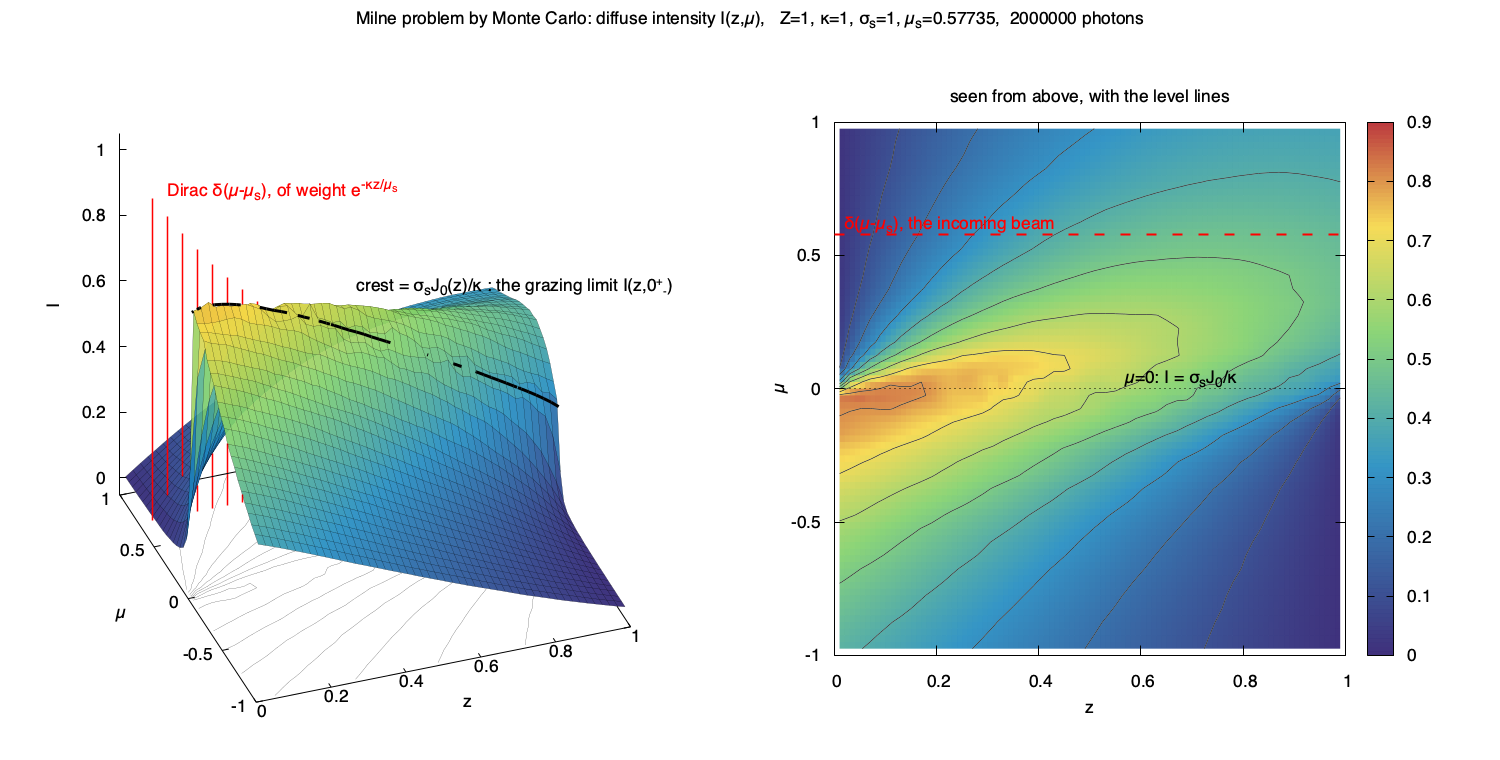
\includegraphics[height=0.78\textheight]{milneMC_I.png}
\end{center}
\vspace{-2mm}
{\scriptsize Left, the surface with the contours projected on the base; right, seen from
above. $Z=1$, $\kappa=\sigma_s=1$, $\mu_s=1/\sqrt3$, $2\times10^6$ photons.}
\end{frame}

%--------------------------------------------------------------------
\begin{frame}{Reading the surface}
\begin{itemize}
\item $I\to0$ on the two \emph{inflow} edges, where the diffuse field has no source:
$z=0$ with $\mu>0$, and $z=Z$ with $\mu<0$.
\item The \textcolor{red}{red impulses} at $\mu=\mu_s$ are the Dirac of the sunlight, of
weight $\e^{-\kappa z/\mu_s}$: it is carried analytically, not sampled. Smeared over one
bin it would stand at $1/\Delta\mu\approx24$ and flatten everything else.
\item The ridge near $\mu\simeq0^-$ at small $z$ is \emph{not} a second Dirac: it is the
grazing radiation backscattered out of the illuminated face.
\item The edge values agree with the emerging intensities computed independently by the
next event estimator: $I(0,-0.975)=0.4217$, $I(Z,0.975)=0.3618$.
\end{itemize}
\end{frame}

%--------------------------------------------------------------------
\begin{frame}{The ridge is the grazing limit}
For the diffuse field,
\[
I(z,\mu)=\frac1{|\mu|}\int S(z')\,\e^{-\kappa|z-z'|/|\mu|}\d z'
\ \xrightarrow[\ \mu\to0\ ]{}\ \frac{S(z)}{\kappa}=\frac{\sigma_sJ_0(z)}{\kappa},
\]
the exponential concentrating on the local source. The crest of the surface must therefore
ride at $\sigma_sJ_0/\kappa$ --- the black line on the figure --- and it does.
\medskip

A smooth monotone rise across the 48 bins, not a peak, and it matches the integral equation:
\begin{center}\small
\begin{tabular}{lccccc}\toprule
$\mu$ & $-0.979$ & $-0.500$ & $-0.104$ & $-0.062$ & $-0.021$\\\midrule
MC $I(0,\mu)$ & 0.4205 & 0.6020 & 0.8067 & 0.8175 & 0.8199\\
exact         & 0.4208 & 0.6020 & 0.8067 & 0.8179 & 0.8194\\\bottomrule
\end{tabular}
\end{center}
\medskip

with $\sigma_sJ_0(0)/\kappa=0.807$ as the $\mu\to0^-$ asymptote. It is the radiation that
scattered once or twice just under the illuminated face and creeps out nearly parallel to
it --- the effect that makes limb darkening, and the reason $I(0,\mu)$ doubles between
normal and grazing exit.
\end{frame}

%--------------------------------------------------------------------
\begin{frame}{But the corner is a true discontinuity}
At $z=0$ the diffuse field has no inflow, $I(0,\mu)=0$ for every $\mu>0$, while
$I(0,\mu)\to S(0)/\kappa\approx0.81$ as $\mu\to0^-$.
\begin{block}{Proposition}
Let $\kappa>0$, $I_0,I_Z>0$ and $S\in C^0([0,Z])$, $S>0$. The solution of the
characteristic equations,
\[
I(z,\mu)={\bf 1}_{\mu>0}\Big[\e^{-\kappa z/\mu}I_0+\int_0^z\frac1\mu
\e^{-\frac\kappa\mu(z-z')}S(z')\d z'\Big]
+{\bf 1}_{\mu<0}\Big[\e^{\frac\kappa\mu(Z-z)}I_Z-\int_z^Z\frac1\mu
\e^{\frac\kappa\mu(z'-z)}S(z')\d z'\Big],
\]
completed by $I(z,0)=S(z)/\kappa$ --- which is the transport equation itself at $\mu=0$ ---
is continuous on $(0,Z)\times[-1,1]$.
\end{block}
Continuity fails at the two corners $(0,0)$ and $(Z,0)$: there are boundary layers of width
$O(|\mu|/\kappa)$ near $z=0$ and $z=Z$. That cliff is what looked like a spike on the
surface.
\end{frame}

%--------------------------------------------------------------------
\begin{frame}{Proof (for $\mu>0$; the case $\mu<0$ is symmetric)}
With $u=(z-z')/\mu$ and $S(z)/\kappa=S(z)\int_0^\infty\e^{-\kappa u}\d u$,
\[
I(z,\mu)-\frac{S(z)}\kappa
=\underbrace{I_0\,\mu\,\e^{-\kappa z/\mu}}_{T_1}
+\underbrace{\int_0^{z/\mu}\e^{-\kappa u}\big[S(z-\mu u)-S(z)\big]\d u}_{T_2}
-\underbrace{S(z)\int_{z/\mu}^{\infty}\e^{-\kappa u}\d u}_{T_3}.
\]
With $M=\max S$ and $\varepsilon>0$, $\delta$ given by the uniform continuity of $S$:
\[
|T_1|\le I_0\mu,\qquad |T_3|\le\frac M\kappa\e^{-\kappa z/\mu},\qquad
|T_2|\le\frac\varepsilon\kappa+\frac{2M}\kappa\e^{-\kappa\delta/\mu}.
\]
Hence on every compact $[a,Z-a]\subset(0,Z)$,
\[
\sup_{z\in[a,Z-a]}\Big|I(z,\mu)-\frac{S(z)}\kappa\Big|
\le I_0\mu+\frac M\kappa\e^{-\kappa a/\mu}+\frac\varepsilon\kappa
+\frac{2M}\kappa\e^{-\kappa\delta/\mu}\ \xrightarrow[\mu\to0^+]{}\ \frac\varepsilon\kappa ,
\]
for every $\varepsilon$, so the supremum tends to $0$; joint continuity follows by adding
$|S(z_n)-S(z_0)|/\kappa$. The bound degrades as $a\to0$: the terms $\e^{-\kappa a/\mu}$ are
not small when $a\lesssim\mu/\kappa$ --- the boundary layers.
\end{frame}

%--------------------------------------------------------------------
\begin{frame}[fragile]{Using the program}
\begin{enumerate}
\item \texttt{cd} to this folder;
\item check that the data at the top of \MC\ suit you;
\item compile and run:
\begin{verbatim}
g++ -O3 -std=c++17 -o MilneMC MilneMC.cpp
./MilneMC N=4000000 Nmu=48
\end{verbatim}
\item \texttt{gnuplot milneMC\_I.gp}, then look at \texttt{milneMC\_I.png}.
\end{enumerate}
\medskip

Parameters as \texttt{key=value} on the command line: \texttt{Z kappa sigmas mus N Nz Nmu
batches seed plot}. Output: \texttt{milneMC\_J0.txt}, \texttt{milneMC\_I.txt}
(columns $z$, $\mu$, $I_{\rm diffuse}$, $I_{\rm diffuse}+$beam),
\texttt{milneMC\_exit.txt}, and the editable script \texttt{milneMC\_I.gp}.
\medskip

{\footnotesize \texttt{col = 4} instead of \texttt{col = 3} at the top of the script puts
the beam back inside the surface, spread over the $\mu$ bin containing $\mu_s$ --- what a
raw track-length tally would have shown.}
\end{frame}

%--------------------------------------------------------------------
\begin{frame}{Conclusion}
\begin{itemize}
\item A dozen lines of random walk solve Milne's problem with no quadrature of the
singular kernel $\E_1$ and no treatment of the Dirac inflow --- it is carried analytically.
\item Verified in three regimes: pure absorption (exact), conservative scattering
($\pm0.1\%$ against the integral equation, balance $1.0000$), and absorbing.
\item The surface shows the physics: two vacuum edges, the grazing plateau
$\sigma_sJ_0/\kappa$, and the genuine corner discontinuity at $(0,0)$ --- which the
Proposition explains and which no amount of refinement will remove.
\end{itemize}
\vfill
{\footnotesize\textbf{Acknowledgement.} \MC, the figures and these slides were produced by
Claude Code (Anthropic, model Opus~5).}
\end{frame}

\end{document}
